\documentclass{article}
\usepackage[utf8]{inputenc}
\usepackage[T1]{fontenc}
\usepackage{graphicx}
\usepackage{hyperref}
\usepackage{geometry}
\geometry{margin=1in}

\title{SILICERNIUM}
\date{Encyclopaedia Britannica (1771)}

\begin{document}
\maketitle

\section*{Historical source}
\textbf{Entry ID:} \texttt{entry-silicernium-2001} \\
\textbf{Volume ID:} 192200899 \\
\textbf{Character Count:} 704

\subsection*{Extracted Text}
SILICERNIUM, among the Romanus was a fault of a private nature, provided for the Great line time after the funeral. It confited of beans, lettues, bread, eggs, \&co. Their eyes laid upon the tomb, and they possibly believed that the died would come out of the repair. What was left was generally burnt on the floor. The word \_Alternate\_ as derived from \_Place and\_ crear, i. e. of figure upon a fleece . Eating what had thus been provided for the dead, was effecemed amark of the small minerible powder. A similar entertainment was made by the Greek sit in the tender of the seaside; but it was ufalal among them to treat the globils with the fragments from the feat of the living. See FUNFAL AND INTERLE.



\section*{Source record}
\begin{itemize}
\item \textbf{Dataset:} \texttt{NationalLibraryOfScotland/encyclopaedia\_britannica\_illustrated}
\item \textbf{Dataset Revision:} \texttt{309f765b1ecc83e0a7f7762e44b4a927a7555443}
\item \textbf{Page ID:} \texttt{britannica:309f765b1ecc83e0a7f7762e44b4a927a7555443:train:2001} \\
  \textbf{Filename:} \texttt{page-2001-93040a5ab362.jpg} \\
  \textbf{Row Index:} 2001 \\
  \textbf{SHA256:} \texttt{93040a5ab3625efc...}
\end{itemize}

\begin{figure}[h]
\centering
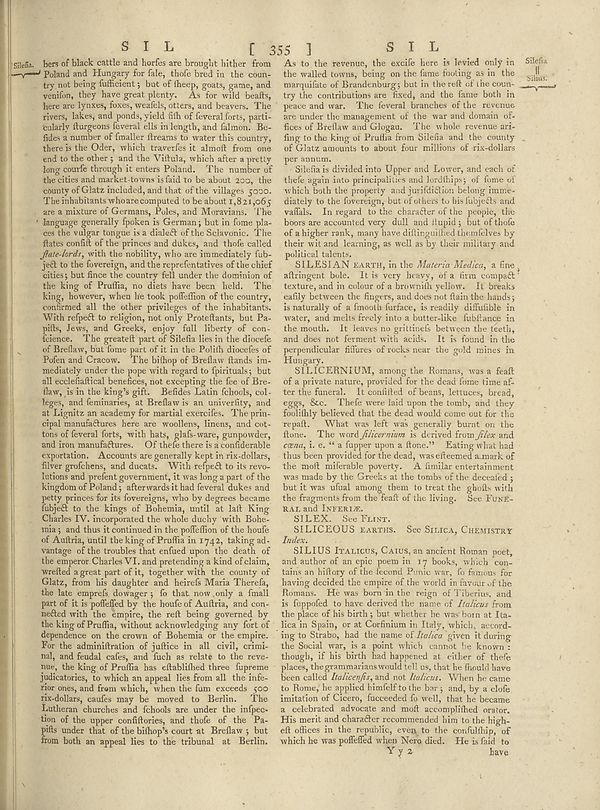
\includegraphics[width=0.85\textwidth]{../scans/page-2001-93040a5ab362.jpg}
\caption*{Source scan: \texttt{page-2001-93040a5ab362.jpg}}
\end{figure}

\end{document}
